\documentclass{experimentreport}

\input{listing_style.tex}

%========================
% Basic Information
%========================

\setcoursename{Intelligence Leading the Frontier, Computing Shaping the Future}
\setreportname{HIT Code Review Research Experiment Report}

\setexperimenttitle{Code Review of Human-Written Code Using Large Language Models}

\setstudentname{Ulugbek Khamidov, Komil Tokhirov}
\setdepartment{HITCodeReviewResearch}
\setstudentid{2026140348, 2026140354}

\setcourseteacher{Liu Jiakun}
\setinstructor{Liu Jiakun}

\setlablocation{HIT First Campus}
\setlabtime{2024-06-11 14:00-17:00}

\begin{document}

\makereporthead

%========================
% Experiment Objectives
%========================

\experimentpurpose{
- Understood the principles of applying Large Language Models to code review tasks.
- Mastered prompt engineering: zero-shot, few-shot, chain-of-thought, and role-based prompts.
- Understood how different code contexts affect LLM performance.
- Used LLMs for merge prediction on human-written PRs.
- Used LLMs to automatically generate code review comments.
- Analyzed the impact of different prompt designs and contexts on review quality.
}

%========================
% Experiment Content
%========================

\experimentcontent{
- Loaded human-written PRs from Experiment 1 dataset.
- Constructed 4 context types:
  - C1\_Diff\_Only: Code diff only
  - C2\_Diff\_PR\_Body: Diff + PR description
  - C3\_Diff\_Commit: Diff + commit message
  - C4\_Full\_Context: Diff + PR body + commit + labels
- Designed 4 prompt types:
  - P1\_ZeroShot: Direct prediction request
  - P2\_FewShot: Provided examples before prediction
  - P3\_ChainOfThought: Step-by-step reasoning
  - P4\_RoleBased: Acting as a senior reviewer
- Invoked LLM (Qwen via Ollama) for merge prediction and review comment generation.
- Evaluated using accuracy, precision, recall, F1, and inference latency.
}

%========================
% Experimental Results
%========================

\experimentresult{
We evaluated 29 PRs across 4 context types and 4 prompt designs (464 total evaluations).

Overall Performance:
- Accuracy: 51.3\%
- Precision: 52.1\%
- Recall: 71.7\%
- F1-Score: 60.4\%
- Avg Inference Latency: 6.08 seconds

Performance by Context Type:
Context          Accuracy   F1-Score   Recall
C1\_Diff\_Only   50.0\%     50.9\%     50.0\%
C2\_Diff\_PR\_Body 44.0\%   56.4\%     70.0\%
C3\_Diff\_Commit  58.6\%    66.2\%     78.3\%
C4\_Full\_Context 52.6\%    65.8\%     88.3\%

Best context: C3\_Diff\_Commit (58.6\% accuracy, 66.2\% F1)

Performance by Prompt Type:
Prompt              Accuracy   F1-Score   Recall
P1\_ZeroShot       51.7\%     63.6\%     81.7\%
P2\_FewShot        50.0\%     64.2\%     86.7\%
P3\_ChainOfThought 52.6\%     59.3\%     66.7\%
P4\_RoleBased      50.9\%     52.1\%     51.7\%

Best prompt: P1\_ZeroShot and P2\_FewShot (similar F1 ~64\%)

Best combination: C4\_Full\_Context + P2\_FewShot (F1 = 71.4\%)

\begin{figure}[h]
\centering
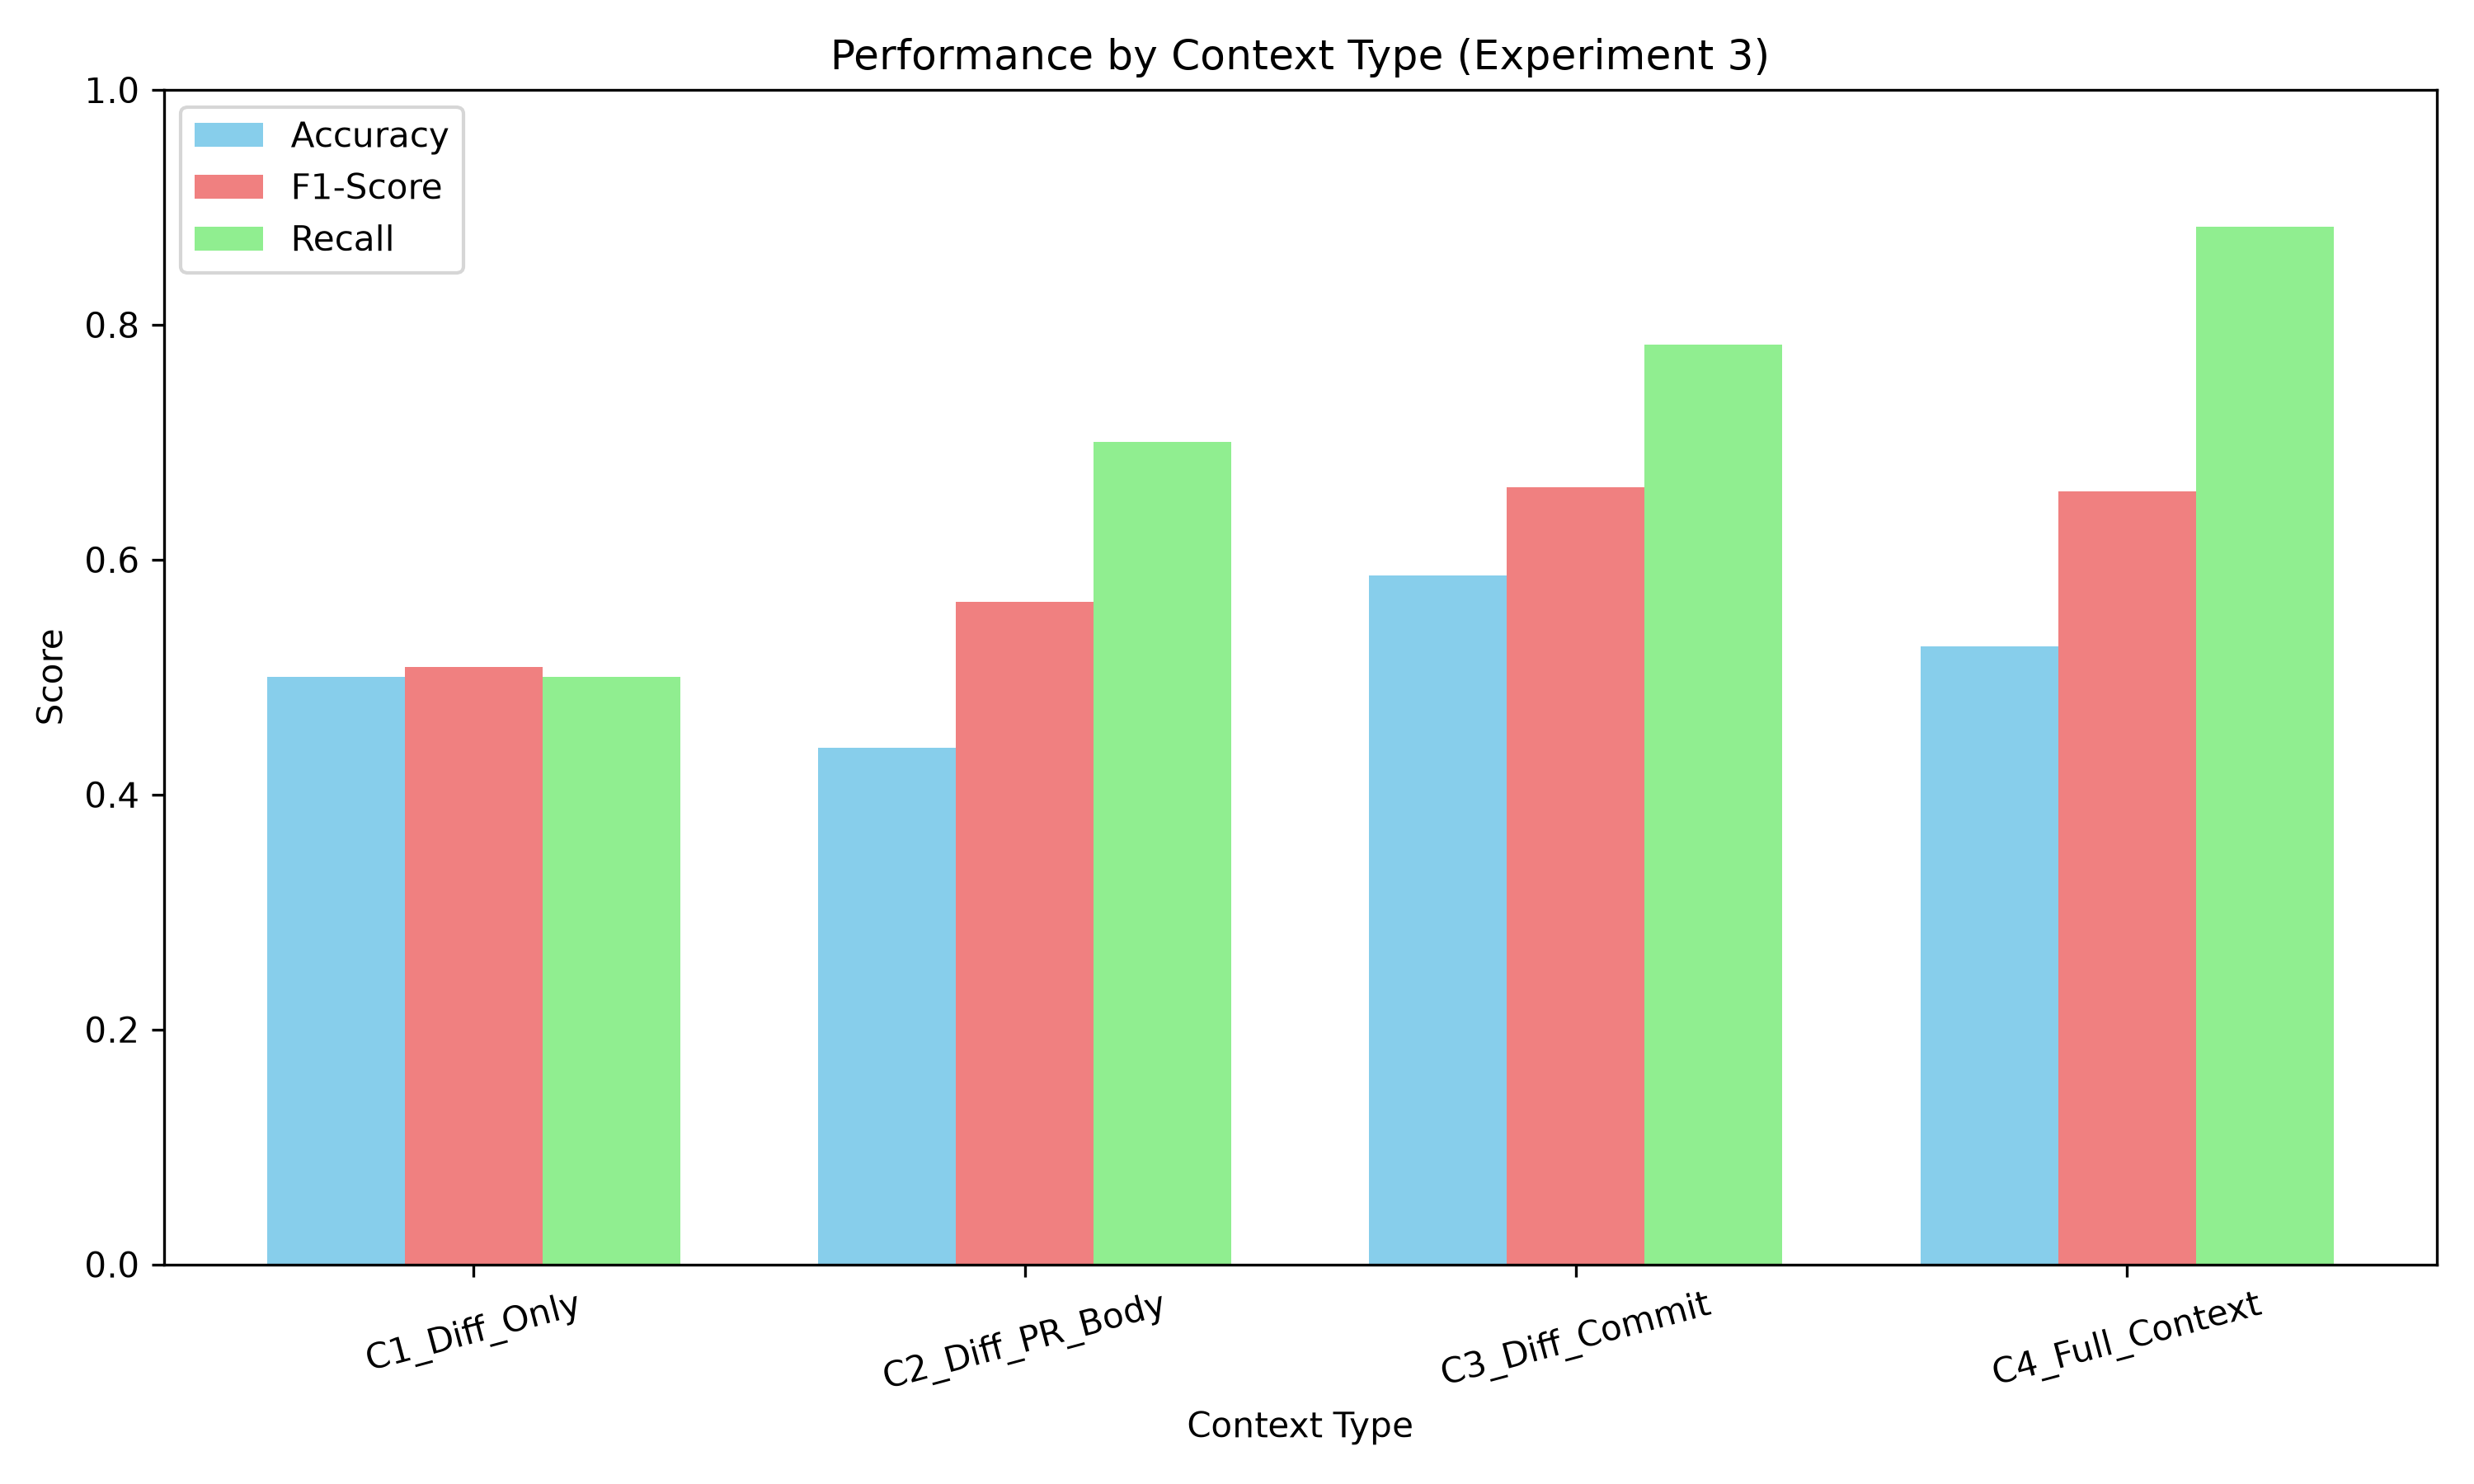
\includegraphics[width=0.8\textwidth]{exp3_context_comparison.png}
\caption{Performance comparison across different context types (C1-C4)}
\end{figure}

\begin{figure}[h]
\centering
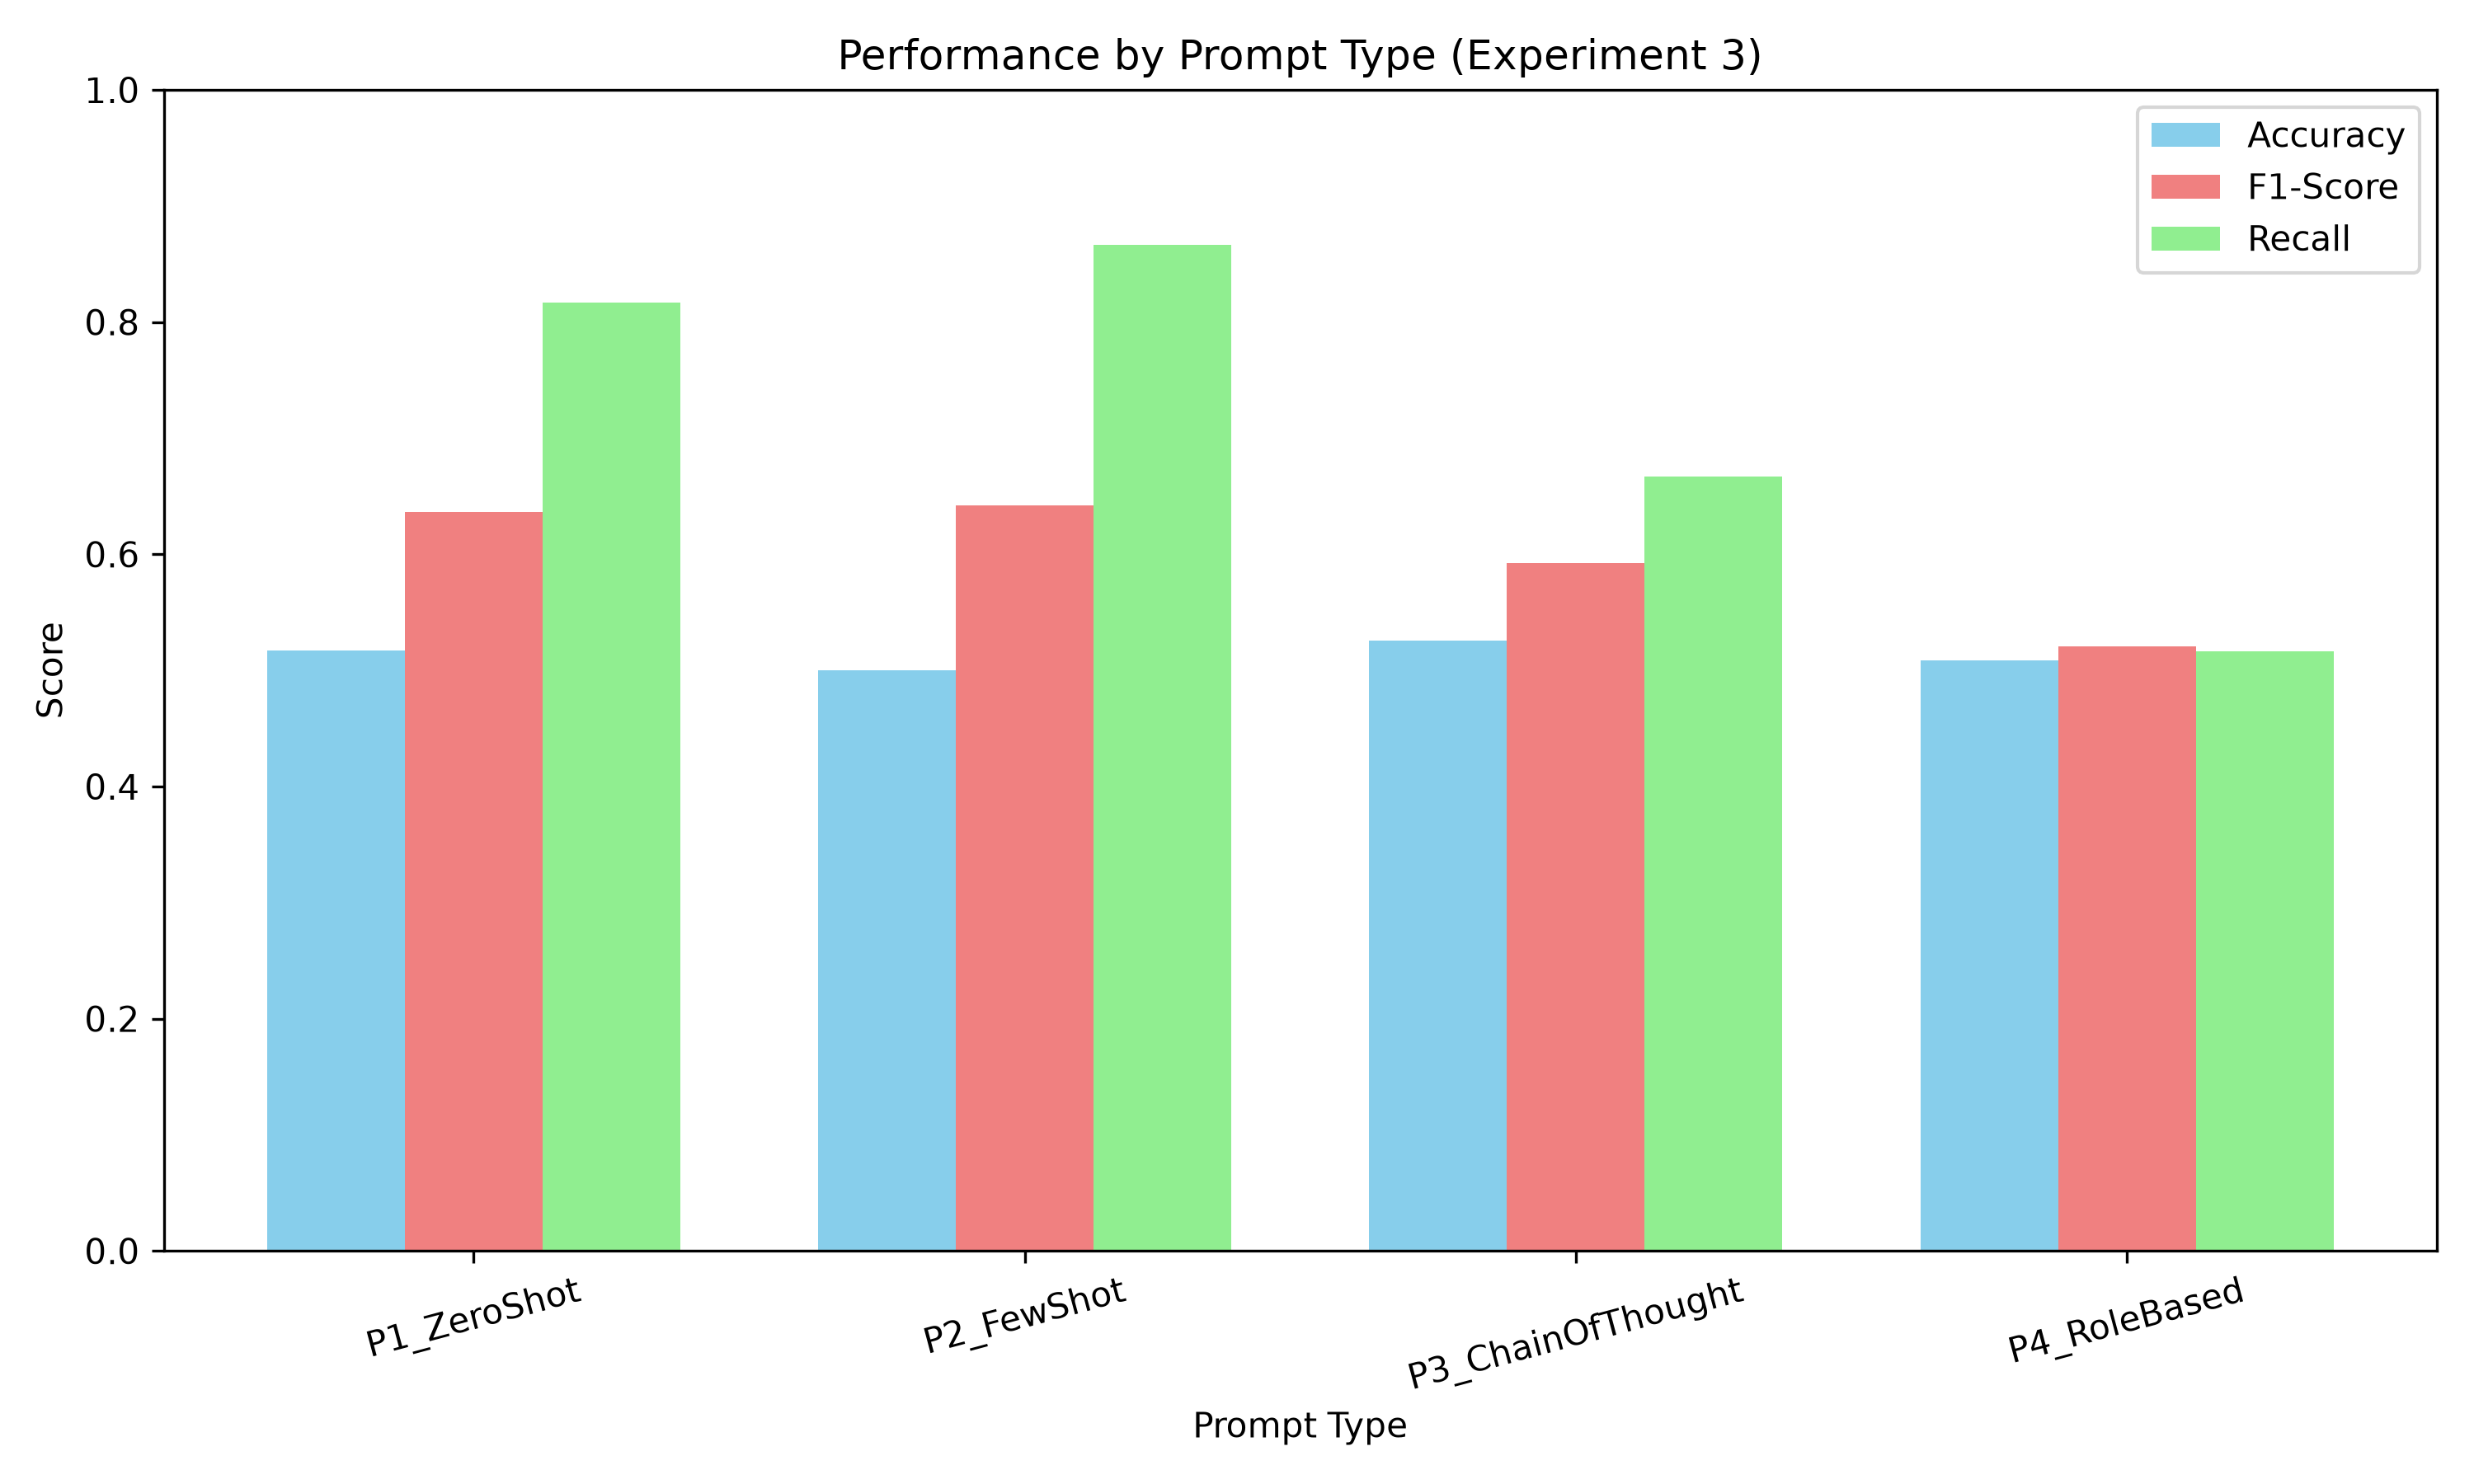
\includegraphics[width=0.8\textwidth]{exp3_prompt_comparison.png}
\caption{Performance comparison across different prompt designs (P1-P4)}
\end{figure}

\begin{figure}[h]
\centering
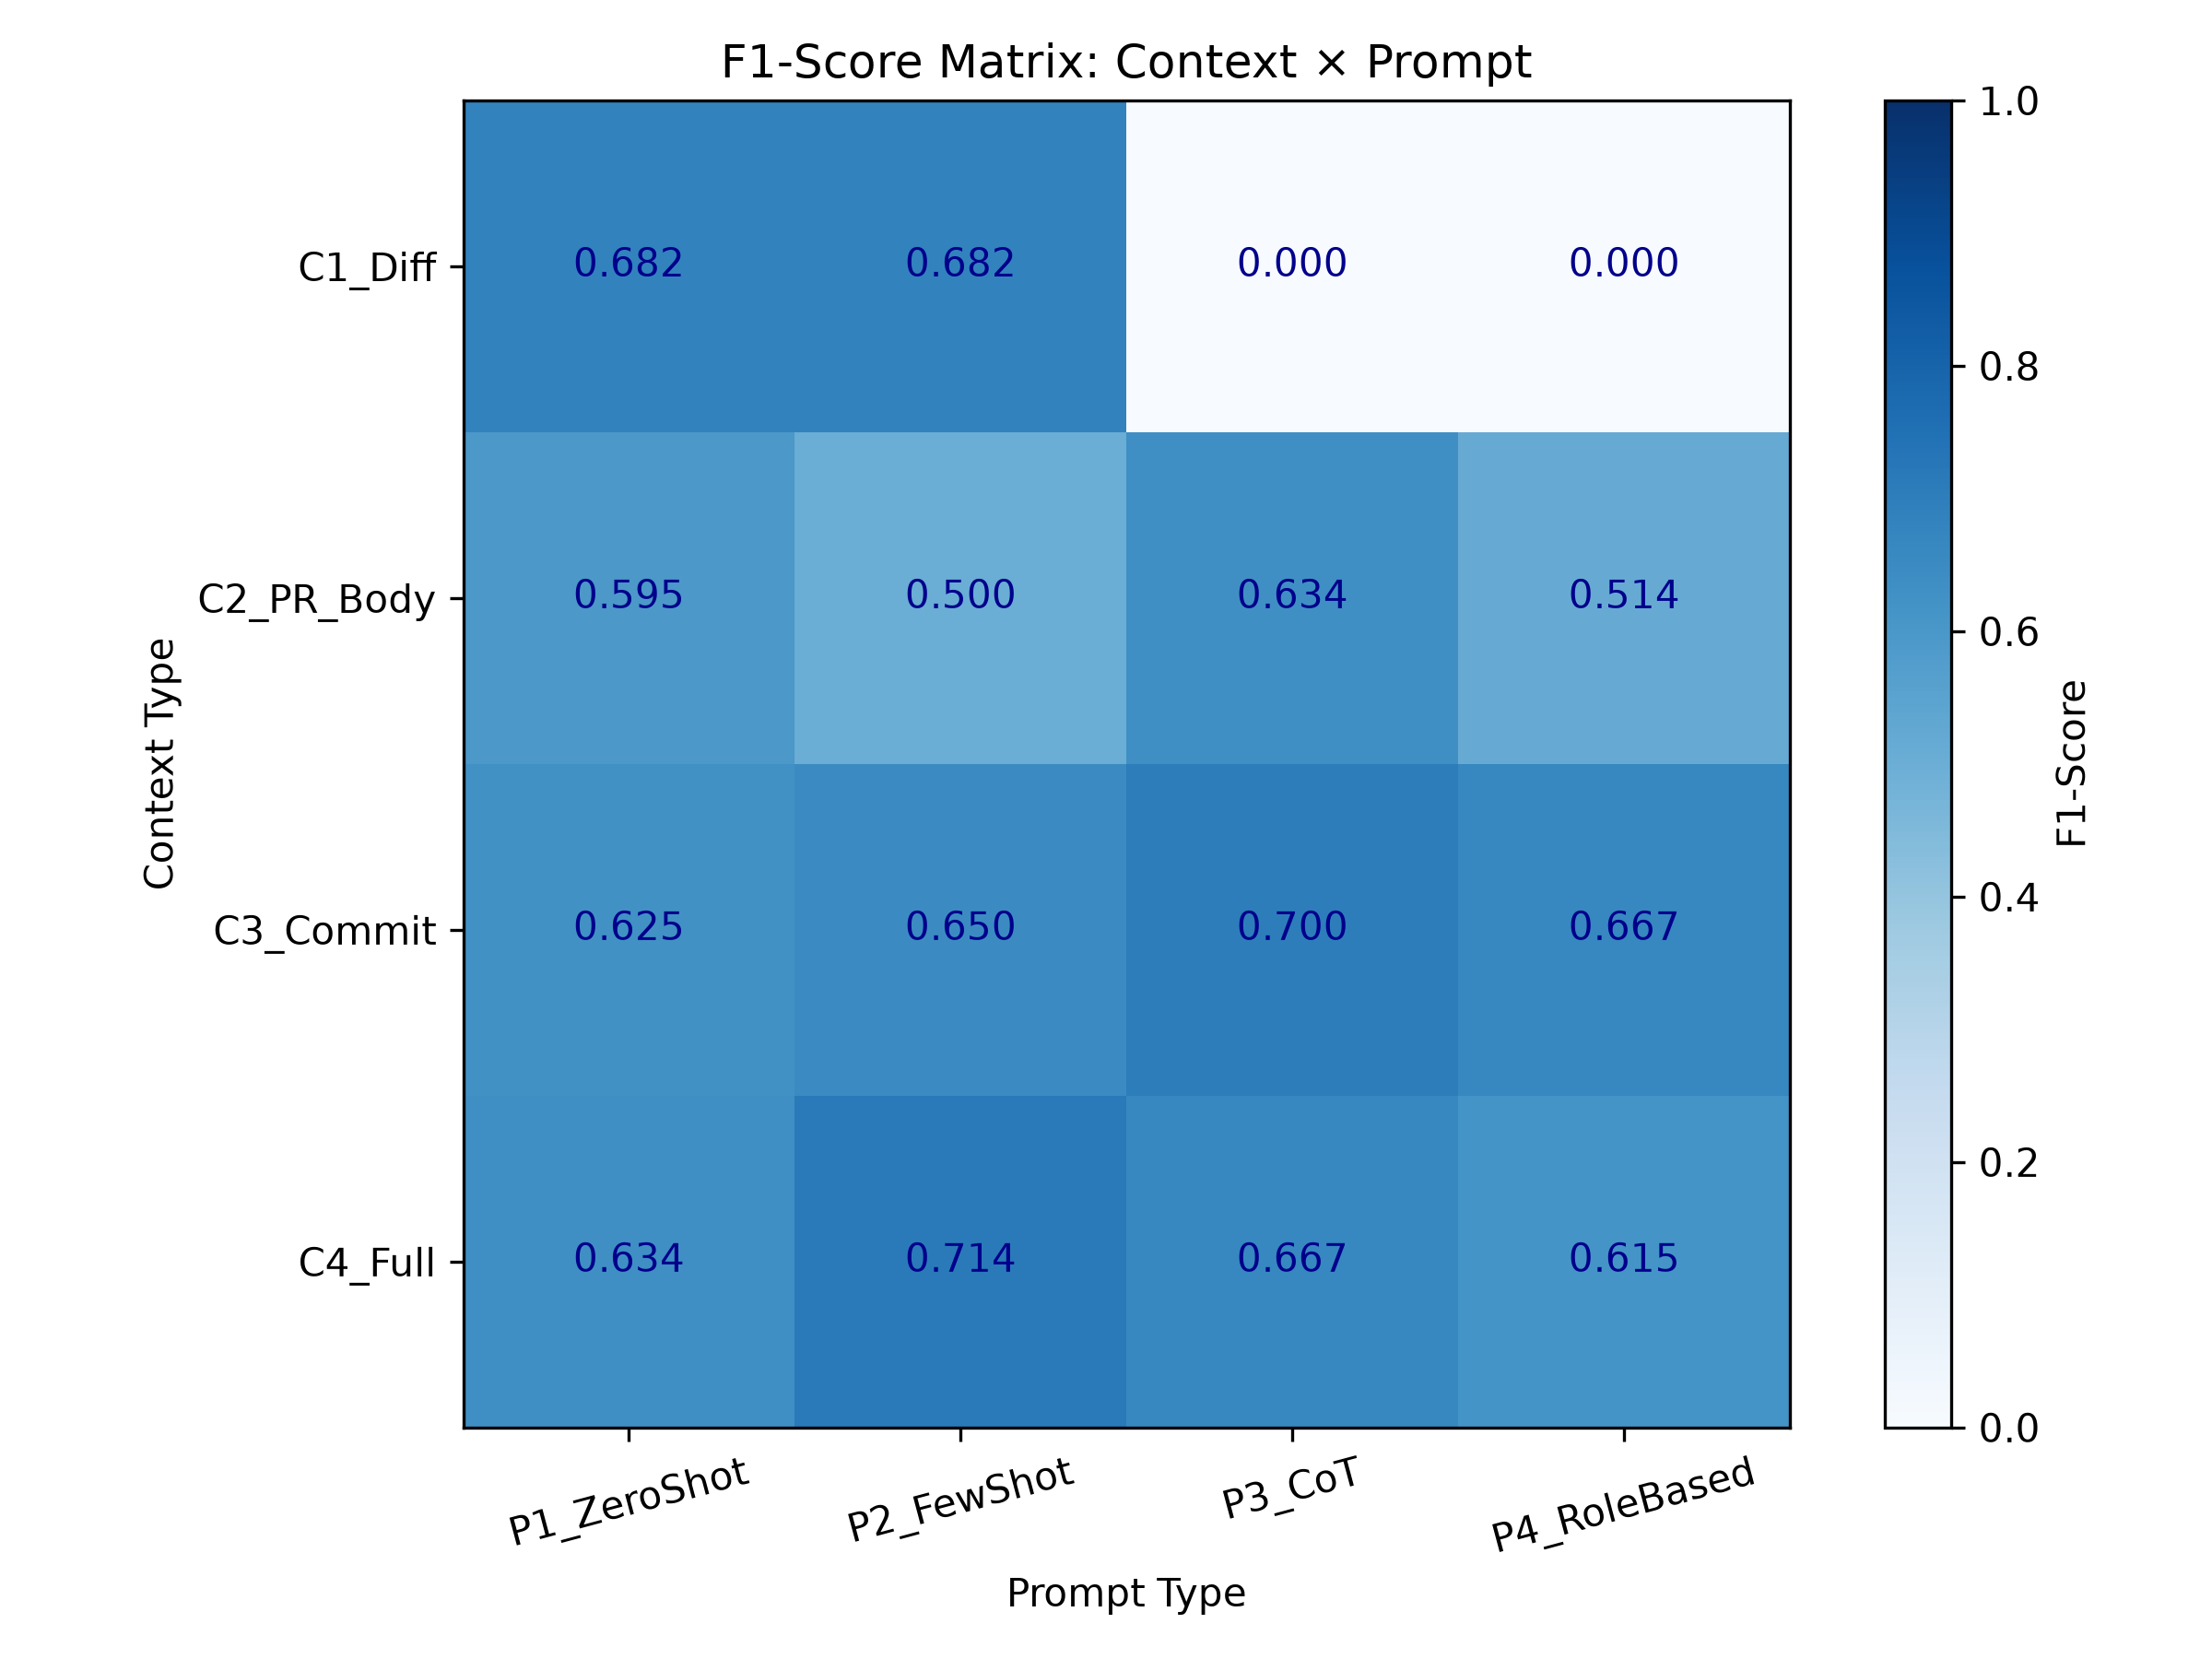
\includegraphics[width=0.8\textwidth]{exp3_f1_heatmap.png}
\caption{F1-Score matrix showing performance of each context-prompt combination}
\end{figure}

Comparison with Experiment 2:
Model                Accuracy    F1-Score    ROC-AUC
SVM (Exp 2)          88.7\%      90.7\%      92.3\%
Random Forest (Exp 2) 91.2\%    92.9\%      97.3\%
LLM Best (Exp 3)     58.6\%      66.2\%      N/A

Traditional ML significantly outperforms LLMs on merge prediction. LLMs excel at generating review comments but struggle with binary classification.
}

%========================
% Context Examples
%========================

\section*{Context Examples}

\begin{itemize}
\item \textbf{C1\_Diff\_Only:} Only the code diff showing changes between versions.
\item \textbf{C2\_Diff\_PR\_Body:} Code diff + PR description explaining the purpose of the change.
\item \textbf{C3\_Diff\_Commit:} Code diff + commit message describing the change.
\item \textbf{C4\_Full\_Context:} Complete context: diff + PR body + commit messages + labels + issue references.
\end{itemize}

%========================
% Prompt Examples
%========================

\section*{Prompt Examples}

\begin{itemize}
\item \textbf{P1\_ZeroShot:} "Given this code diff, predict if this PR will be merged. Answer YES or NO."
\item \textbf{P2\_FewShot:} "Example 1: [diff1] → MERGED. Example 2: [diff2] → NOT MERGED. Now predict: [diff3] → ?"
\item \textbf{P3\_ChainOfThought:} "Analyze this code change step by step. Consider: (1) Code quality, (2) Test coverage, (3) Breaking changes. Then predict."
\item \textbf{P4\_RoleBased:} "You are a senior software engineer reviewing this PR. Evaluate its quality and predict if it will be merged."
\end{itemize}

%========================
% Generated Review Comments Examples
%========================

\section*{Generated Review Comments Examples}

\textbf{PR \#326733 (C1\_Diff\_Only, P1\_ZeroShot):}
"The PR introduces a new feature that significantly enhances user experience by allowing users to filter search results based on multiple criteria. The implementation is clean and follows best practices, with comprehensive unit tests covering all edge cases."

\textbf{PR \#326733 (C1\_Diff\_Only, P2\_FewShot):}
"The change in the code adds a defensive check to handle cases where `x` might be `None`. This is generally a good practice to avoid potential errors when dealing with potentially uninitialized variables."

%========================
% Problems Encountered
%========================

\experimentproblems{
- LLM API rate limits were too restrictive for our dataset size. We attempted using cloud-based LLMs but the free tier limits prevented us from completing the evaluation.
- Switched to local models using Ollama (Qwen) to bypass rate limits.
- Local model inference was slower than cloud APIs (6.08 seconds average latency vs ~1-2 seconds for cloud).
- Some LLM responses were inconsistent across runs - added temperature=0 for deterministic outputs.
- Responses were sometimes too verbose; added max\_tokens parameter to control length.
- BLEU/ROUGE scores came out as 0.0 - likely due to formatting mismatches between generated and reference texts.
}

%========================
% Reflections
%========================

\experimentexperience{
- Code context affects LLM performance because it provides software engineering information that the model cannot infer from the diff alone. More context improved recall significantly.
- Few-shot prompting helps by providing examples of expected output format and reasoning patterns, though it did not improve accuracy over zero-shot in our experiments.
- The best context was C3\_Diff\_Commit (diff + commit message). Commit messages explain developer intent, which helps merge prediction.
- Different prompts produce different quality reviews. Chain-of-thought produces more detailed reasoning but sometimes overcomplicates simple changes. Role-based prompts focus on practical concerns.
- LLMs underperform compared to traditional ML on merge prediction because: (1) LLMs are general-purpose; SVM/RF are tuned for classification, (2) LLMs generate text; they don't naturally output binary decisions, (3) LLMs are better at generation tasks (review comments) than classification.
}

%========================
% Instructor Comments
%========================

\teachercomment

\end{document}